\section{Test af accelerometer} 
\label{sec:test_acc}
I dette projekt anvendes to accelerometer som sensorer til opsamling af signaler. For at kunne anvende et accelerometer er det vigtigt at kende forskellige tolerancer i forhold til deres datablade, hvorfor et forsøg udføres for at kunne tage højde for disse parametre.

\subsection{Formål}
Denne test har til formål at identificere spændingen i henholdsvis $0^{\circ}$ og $90^{\circ}$, hvorudfra vinkler kan beregnes. Derudover identificeres støjsignaler i outputsignalet samt offsettet og sensitiviteten, så dette kan tages højde for i pilotforsøget \autoref{sec:pilotforsoeg} og senere forsøg.

\begin{enumerate}
\item Identificering af støj i outputsignaler for accelerometrene
\item Identificering af offsettet og sensitiviteten for accelerometrene
\item Identificering af spænding ved $0^{\circ}$ og $90^{\circ}$
\end{enumerate}

\subsection{Materialer}
\begin{itemize}
\item Accelerometre ADXL$335$
\item Tape
\item Vinkel
\item Vaterpas
\item Breadboard
\item Computer med Scopelogger og MATLAB
\item NI USB-6009
\end{itemize}

\subsection{Metode}
\begin{enumerate}
\item Der foretages målinger i accelerometerets tre akser og i de seks positioner som accelerometeret, hvorved støj som accelerometeret påvirkes med kan identificeres.
\item Ud fra de øvrige målinger kan offset og sensitiviteten beregnes ved at se på de akser hvor accelerometeret udsættes for 0 g-påvirkning  . 
\item Spændingen ved $0^(\circ}$ og $90^{\circ}$ beregnes ved at måle påvirkningen af accelerometeret derefter dividere afvigelsen af denne med 90 for at finde for 1 grads g-påvirkning, hvorefter påvirkningen kan ganges med den ønskede vinkel. 
\end{enumerate}

\subsection{Forsøgsopstilling}
Forsøgsopstillingen udføres på samme måde for begge accelerometre.
\begin{itemize}
\item Accelerometeret tilkobles breadboardet og sættes fast med tape.
\item Accelerometeret indstilles så det er vinkelret
\begin{itemize}
\item Accelerometeret placeres efter fremgangsmåden for hver øvelse, som er illustreret i \autoref{sec:acc_fremgangsmaade}
\end{itemize}
\item Accelerometeret tilkobles NI USB-6009
\item NI USB-6009 tilkobles computer
\end{itemize}

\subsection{Fremgangsmåde} 
\label{sec:acc_fremgangsmaade}
Der foretages seks forskellige positioner for hvert accelerometer. Hver position måles tre gange og samles i 10 sekunder ved 100 Hz, hvilket er det dobbelte af båndbredden for accelerometrene \citep{analogdevices2010}. De forskellige fremgangsmåder er illustreret på \autoref{fig:acc_paavirkning}. 
\begin{itemize}
\item Accelerometeret er lodret opad
\item Accelerometeret er lodret nedad
\item Accelerometeret er vandret mod højre
\item Accelerometeret er vandret mod venstre
\item Accelerometeret er plan på bordet opad
\item Accelerometeret er plan på bordet nedad
\end{itemize}

\begin{figure}[H]
\centering
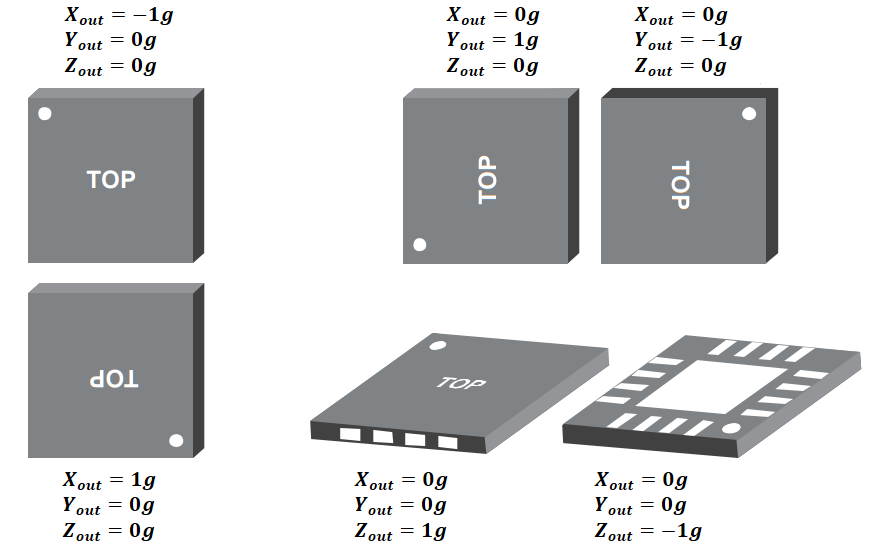
\includegraphics[width=0.3\textwidth]{figures/acc_paavirkning}
\caption{Påvirkning af accelerometeret i forskellige positioner. Til venstre måles accelerometeret i lodret plan, til højre øverst vandret og til højre nederst i plan \citep{analogdevices2010}}
\label{fig:acc_paavirkning}
\end{figure}

\subsection{Resultater}
Der er foretaget en fourier transformations analyse (FFT) af de tre målinger foretaget i de seks positioner for at identificeres støj. Ud fra resultaterne ses det at der på begge accelerometre er støj ved 33-34Hz. En af målingerne fremgår på \autoref{fig:FFT_acc}. 

\begin{figure}[H]
\centering
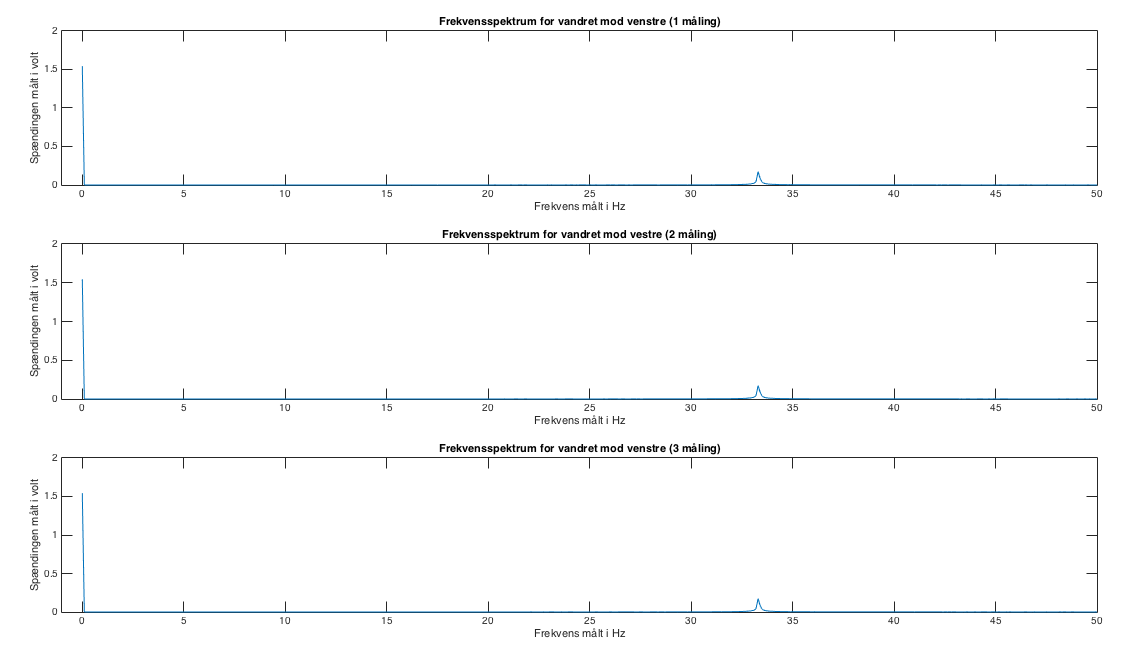
\includegraphics[width=0.3\textwidth]{figures/FFT_acc}
\caption{FFT analyse af de tre målinger for det ene accelerometer målt i vandret mod venstre, hvor accelerometeret bliver påvirket i y-aksens retning}
\label{fig:FFT_acc}
\end{figure}

Ud fra de tre målinger foretaget i de forskellige positioner beregnes dengennemsnitlige værdi af målingerne på de forskellige akser, herefter plottes disse i en graf, hvorved det er muligt at se hvilken akse der bliver påvirket mest under øvelsen. Målingerne fremgår på \autoref{fig:paavirkning}. 

\begin{figure}[H]
\centering
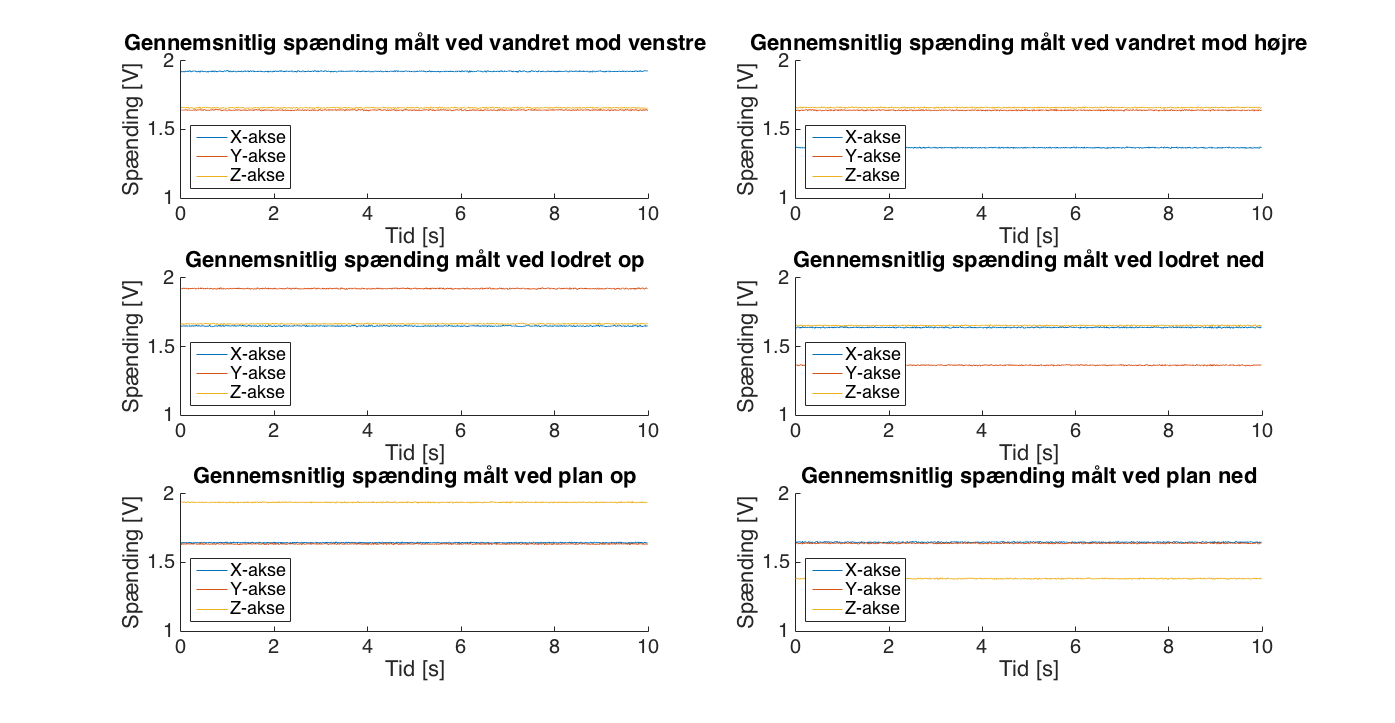
\includegraphics[width=0.3\textwidth]{figures/paavirkning}
\caption{Påvirkningen af accelerometerets tre akser ved de seks forskellige positioner}
\label{fig:paavirkning}
\end{figure}

Der beregnes offset ud fra målingerne hvor accelerometeret påvirkes med 0 g. Der hvor accelerometeret er påvirket med 0 g er illustreret på \autoref{fig:acc_paavirkning}. Målingerne fremgår af \autoref{Tab:acc_offset}. 

\begin{table}[H]
	\centering
	\begin{tabular}{|l|l|l|}
	\textbf{Målt retning} & \textbf{Målt akse} & \textbf{Offset} \\ \hline
    \textbf{Lodret op} 		& X 		& $1,6793~V$ 	\\ \hline
    \textbf{Lodret op} 		& Z 		& $1,6857~V$ 	 \\ \hline
    \textbf{Lodret ned}		& X 		& $1,6750~V$ 	\\ \hline
    \textbf{Lodret ned}		& Z 		& $1,6806~V$  	\\ \hline
    \textbf{Vandret højre} 	& Y 		& $1,6760~V$    \\ \hline     
    \textbf{Vandret højre} 	& Z 		& $1,6828~V$ 	\\ \hline
    \textbf{Vandret venstre}	& Y 		& $1,6755~V$ 	\\ \hline
    \textbf{Vandret venstre}	& Z 		& $1,6836~V$		\\ \hline
    \textbf{Plan op} 		& X 		& $1,6773~V$		\\ \hline		
    \textbf{Plan op} 		& Y 		& $1,6734~V$    \\ \hline
    \textbf{Plan ned} 		& X 		& $1,6787~V$		\\ \hline
    \textbf{Plan ned} 		& Y 		& $1,6755~V$		\\ \hline
	\end{tabular}
	\caption{Offsettet beregnet for de forskellige akser hvor accelerometeret udsættes for en 0 g-påvirkning}
	\label{Tab:acc_offset}
\end{table}

Der beregnes sensitiviten ud fra forskellen mellem 0 og 1 g-påvirkningen af accelerometeret. Der hvor accelerometeret er påvirket med 1 g er illustreret på \autoref{fig:acc_paavirkning}. Målingerne fremgår af \autoref{Tab:acc_sensitiviteten}. 

\begin{table}[H]
	\centering
	\begin{tabular}{|l|l|l|}
	\textbf{Målt retning} & \textbf{Målt akse} & \textbf{Sensitivitet} \\ \hline
    \textbf{Lodret op} 		& Y		& $0,1232~V/g$ 	\\ \hline
    \textbf{Lodret ned}		& Y 		& $-0,1079~V/g$ 	\\ \hline
    \textbf{Vandret højre} 	& X 		& $0,1092~V/g$     \\ \hline     
    \textbf{Vandret venstre}	& X 		& $-0,1164~V/g$ 	\\ \hline
    \textbf{Plan op} 		& Z 		& $0,1130~V/gV$    	\\ \hline		
    \textbf{Plan ned} 		& Z 		& $-0,1167~V/g$		\\ \hline
	\end{tabular}
	\caption{Sensitiviteten beregnet for de forskellige akser hvor accelerometeret udsættes for en 1 g-påvirkning}
	\label{Tab:acc_offset}
\end{table}

Ud fra senstitivten beregnes spændingen ved $1^{\circ}$ og $90^{\circ}$ i negativ og positiv retning\fxnote{Er der nødvendig med 1 grad?}. Spændingen svarende til $0^{\circ}$ svarer til den målte offsetværdi som fremgår af \autoref{Tab:acc_offset}. Beregningerne af spændingen ved de valgte grader fremgår af \autoref{Tab:acc_grader} og er beregnet ud fra følgende ligning:

\begin{equation}
	V_{out} = V_{offset} + sensitiviteten \cdot \sin(vinklen) \\
\end{equation}

 \begin{table}[H]
	\centering
	\begin{tabular}{|l|l|l|l|}
	\textbf{Målt retning} & \textbf{Målt akse} & \textbf{Spændingen ved grad} & \textbf{Spændingen ved 90 grader} \\ \hline
    \textbf{Positiv} 	& Y		& $1,7985~V$   	&	$12,7589~V$\\ \hline
    \textbf{Negativ}		& Y		& $1,5692~V$  	&	$-8,0339~V$\\ \hline
    \textbf{Positiv} 	& X 		& $1,7917~V$   	& 	$11,5105~V$ \\ \hline     
    \textbf{Negativ}		& X 		& $1,5614~V$		&	$-8,7982~V$\\ \hline
    \textbf{Positiv} 	& Z 		& $1,7924~V$   	& 	$11,8494~V$	\\ \hline		
    \textbf{Negativ} 	& Z 		& $1,5629~V$		&	$-8,8190~V$ \\ \hline
	\end{tabular}
	\caption{Beregnet spænding ved henholdvis 1 og 90 grader i positiv og negativ retning}
	\label{Tab:acc_grader}
\end{table}





